%!TEX root = ../main.tex

\begin{frame}{Resultados e Discussão}
 \begin{itemize}
   \item Estimação de idade a partir de uma imagem de face
   \ \ \newline
    \item Arquiteturas
    \begin{itemize}
      \item LeNet
      \item AlexNet
      \item VGG-16
      \item SqueezeNet
    \end{itemize}
   \ \ \newline
   \item \alert{9 Abordagens}
   \end{itemize}
\end{frame}


\begin{frame}{Abordagem 1: LeNet e AlexNet com Imagens Normalizadas}
 \begin{itemize}
   \item Entradas: Imagens normalizadas
   \item Redes: LeNet e AlexNet
   \item Funções de ativação: \emph{ReLU} e \emph{Leaky ReLU}
   \end{itemize}
\end{frame}

\begin{frame}{Abordagem 1: LeNet e AlexNet com Imagens Normalizadas}
\begin{figure}[h!]
  \caption{Resultados do treinamento e teste da CNN LeNet \emph{ReLU}.}
  \begin{subfigure}[hb]{0.4\textwidth}
    \caption{RMSE de treinamento.}
    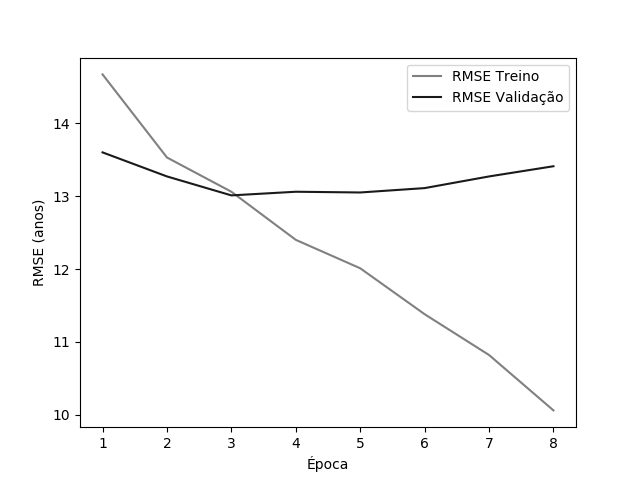
\includegraphics[width=\linewidth]{img/graficos/history/lenet/fig-history-image-treat-1-lenet-relu-rmse.png}%
  \end{subfigure}%
  \begin{subfigure}[hb]{0.4\textwidth}
    \caption{Reta-0 do conjunto de teste.}
    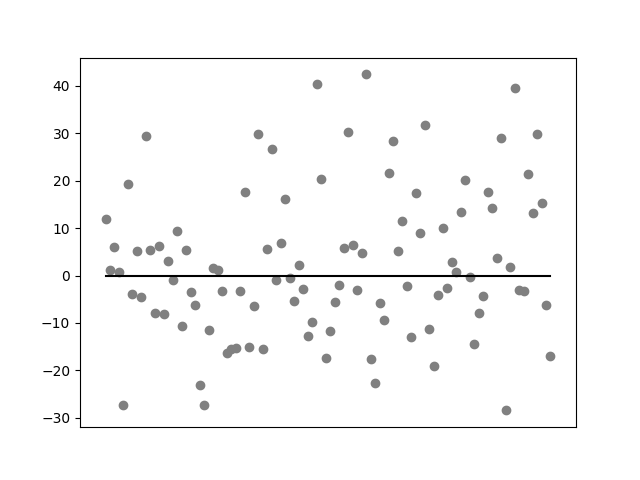
\includegraphics[width=\linewidth]{img/graficos/reta0/lenet/fig-reta-0-image-treat-1-lenet-relu.png}%
  \end{subfigure}
\end{figure}
\end{frame}

\begin{frame}{Abordagem 1: LeNet e AlexNet com Imagens Normalizadas}
  \begin{figure}[h!]
    \caption{Resultados do treinamento e teste da CNN LeNet \emph{Leaky ReLU}.}
  \begin{subfigure}[hb]{0.4\textwidth}
    \caption{RMSE de treinamento.}
    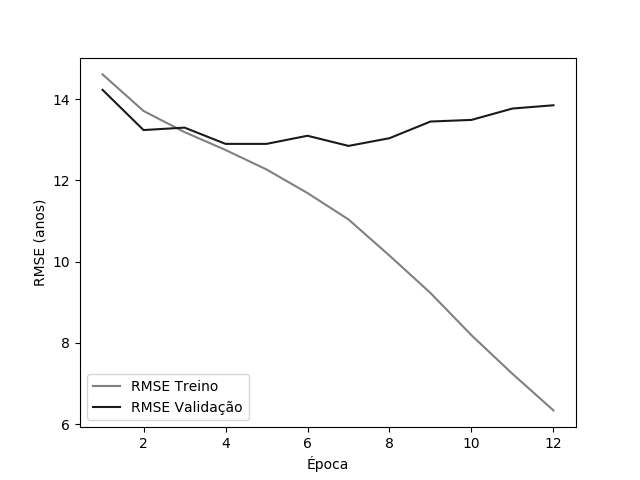
\includegraphics[width=\linewidth]{img/graficos/history/lenet/fig-history-image-treat-1-lenet-lrelu-rmse.png}
  \end{subfigure}
  \begin{subfigure}[hb]{0.4\textwidth}
    \caption{Reta-0 do conjunto de teste.}
   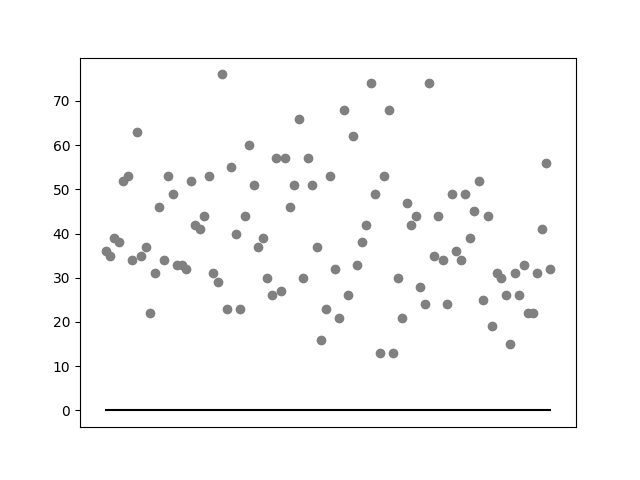
\includegraphics[width=\linewidth]{img/graficos/reta0/lenet/fig-reta-0-image-treat-1-lenet-lrelu.png}
  \end{subfigure}%
\end{figure}
\end{frame}

\begin{frame}{Abordagem 1: LeNet e AlexNet com Imagens Normalizadas}
  \begin{figure}[ht!]
    \caption{Resultados do treinamento e teste da CNN AlexNet \emph{ReLU} de acordo com a Abordagem 1.}\label{fig:alexnet-abordagem1}
    \begin{subfigure}[hb]{0.4\linewidth}
      \caption{RMSE Treinamento.}

      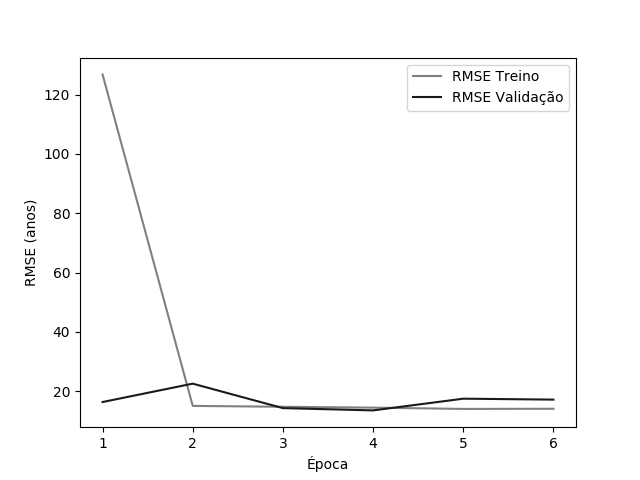
\includegraphics[width=\linewidth]{img/graficos/history/alexnet/fig-history-image-treat-1-alexnet-relu-rmse.png}
    \end{subfigure}
    \begin{subfigure}[hb]{0.4\linewidth}
      \caption{Reta-0.}
      \label{fig:reta0reludying}
      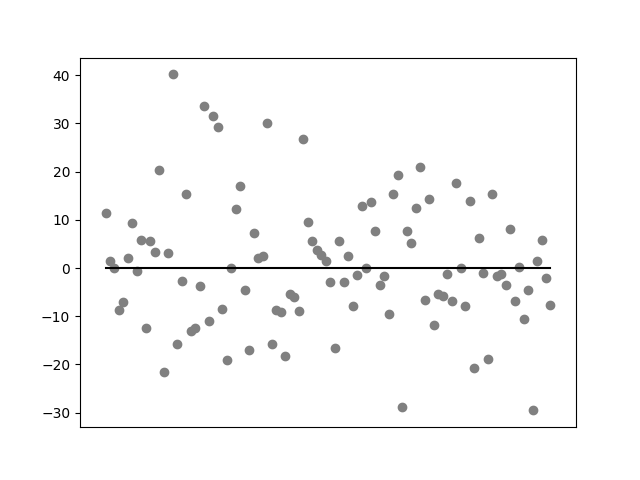
\includegraphics[width=\linewidth]{img/graficos/reta0/alexnet/fig-reta-0-image-treat-1-alexnet-relu.png}%
    \end{subfigure}
\end{figure}
\end{frame}

\begin{frame}{Abordagem 1: LeNet e AlexNet com Imagens Normalizadas}
  \begin{figure}[ht!]
    \caption{Resultados do treinamento e teste da CNN AlexNet \emph{Leaky ReLU} de acordo com a Abordagem 1.}\label{fig:alexnet-abordagem1}
    \begin{subfigure}[hb]{0.4\linewidth}
      \caption{RMSE Treinamento.}
      \label{fig:histalexlrelunorm}
      \centering
      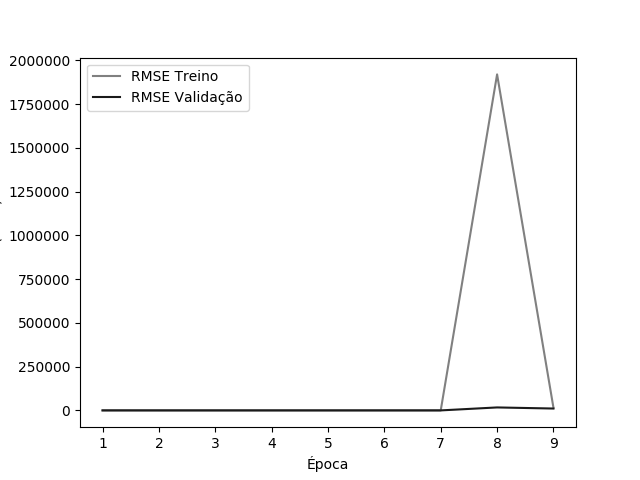
\includegraphics[width=\linewidth]{img/graficos/history/alexnet/fig-history-image-treat-1-alexnet-lrelu-rmse.png}
    \end{subfigure}
    \begin{subfigure}[hb]{0.4\linewidth}
      \caption{Reta-0.}

      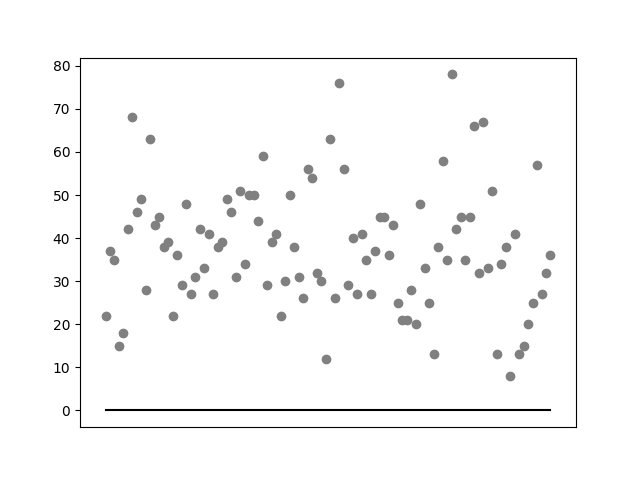
\includegraphics[width=\linewidth]{img/graficos/reta0/alexnet/fig-reta-0-image-treat-1-alexnet-lrelu.png}
    \end{subfigure}%
\end{figure}
\end{frame}

\begin{frame}{Abordagem 1: LeNet e AlexNet com Imagens Normalizadas}
  \begin{table}[!ht]
		\caption{Resultados do treino e teste dos modelos propostos na Abordagem 1.}
		\label{tab:results-1}
		\begin{center}
			\begin{tabular}{l l l l l}
				\toprule
				Rede & Função de ativação & Épocas & MAE Teste & RMSE Teste \\
				\midrule
				LeNet & \emph{ReLU}  & 4 & 10.53 & 13.55 \\
				LeNet & \emph{Leaky ReLU} & 8 & 38.33 & 40.82 \\
				AlexNet & \emph{ReLU}  & 5 & 11.03 & 13.76 \\
				AlexNet & \emph{Leaky ReLU} & 5 & 39.27 & 41.97 \\
				\bottomrule
			\end{tabular}
		\end{center}
	\end{table}
\end{frame}





\begin{frame}{Abordagem 2}
 \begin{itemize}
   \item Entradas: Imagens normalizadas, \alert{\emph{data augmentation}}
   \begin{itemize}
     \item Rotação, zoom, inversçao horizontal e translação
   \end{itemize}
   \item Redes: LeNet e AlexNet
   \item Funções de ativação: \emph{ReLU} e \emph{Leaky ReLU}
   \end{itemize}
\end{frame}

\begin{frame}{Abordagem 2: Introduzindo \emph{Data Augmentation}}
\begin{figure}[h!]
  \caption{Resultados do treinamento e teste da CNN LeNet \emph{ReLU}.}
  \begin{subfigure}[hb]{0.4\textwidth}
    \caption{RMSE de treinamento.}
    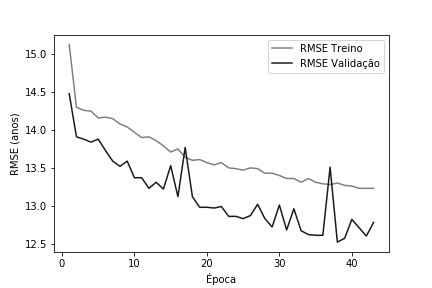
\includegraphics[width=\linewidth]{img/graficos/history/lenet/fig-history-image-treat-2-lenet-relu-rmse.png}%
  \end{subfigure}%
  \begin{subfigure}[hb]{0.4\textwidth}
    \caption{Reta-0 do conjunto de teste.}
    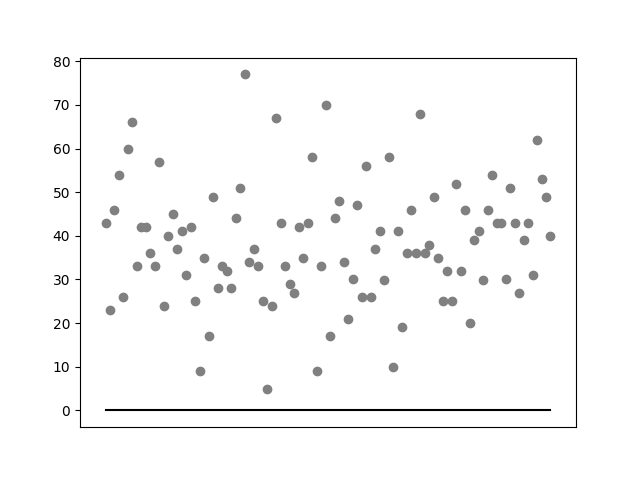
\includegraphics[width=\linewidth]{img/graficos/reta0/lenet/fig-reta-0-image-treat-2-lenet-relu.png}%
  \end{subfigure}
\end{figure}
\end{frame}

\begin{frame}{Abordagem 2: Introduzindo \emph{Data Augmentation}}
  \begin{figure}[h!]
    \caption{Resultados do treinamento e teste da CNN LeNet \emph{Leaky ReLU}.}
  \begin{subfigure}[hb]{0.4\textwidth}
    \caption{RMSE de treinamento.}
    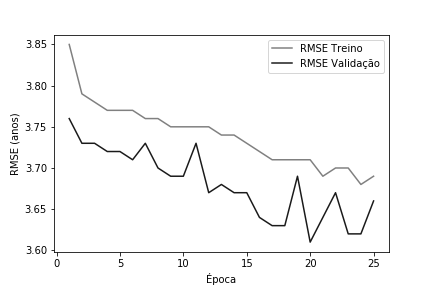
\includegraphics[width=\linewidth]{img/graficos/history/lenet/fig-history-image-treat-2-lenet-lrelu-rmse.png}
  \end{subfigure}
  \begin{subfigure}[hb]{0.4\textwidth}
    \caption{Reta-0 do conjunto de teste.}
   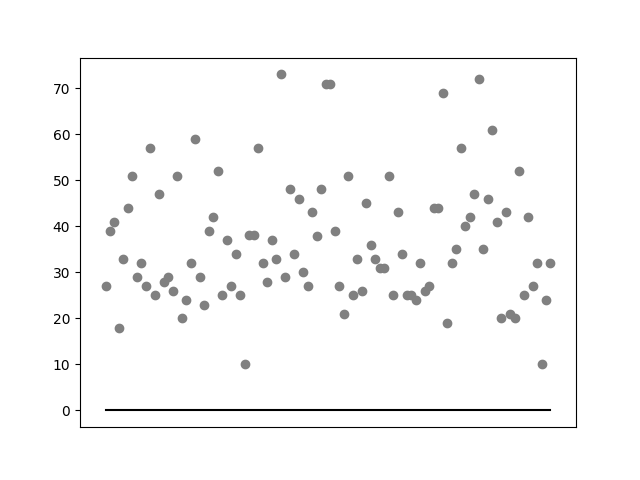
\includegraphics[width=\linewidth]{img/graficos/reta0/lenet/fig-reta-0-image-treat-2-lenet-lrelu.png}
  \end{subfigure}%
\end{figure}
\end{frame}

\begin{frame}{Abordagem 2: Introduzindo \emph{Data Augmentation}}
  \begin{figure}[ht!]
    \caption{Resultados do treinamento e teste da CNN AlexNet \emph{ReLU} de acordo com a Abordagem 2.}\label{fig:alexnet-abordagem1}
    \begin{subfigure}[hb]{0.4\linewidth}
      \caption{RMSE Treinamento.}

      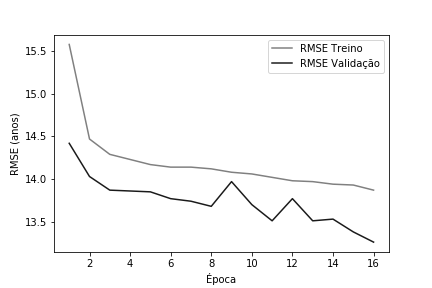
\includegraphics[width=\linewidth]{img/graficos/history/alexnet/fig-history-image-treat-2-alexnet-relu-rmse.png}
    \end{subfigure}
    \begin{subfigure}[hb]{0.4\linewidth}
      \caption{Reta-0.}
      \label{fig:reta0reludying}
      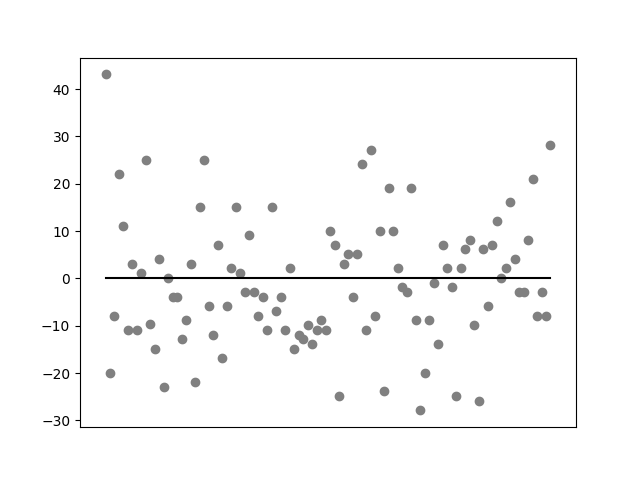
\includegraphics[width=\linewidth]{img/graficos/reta0/alexnet/fig-reta-0-image-treat-2-alexnet-relu.png}%
    \end{subfigure}
\end{figure}
\end{frame}

\begin{frame}{Abordagem 2: Introduzindo \emph{Data Augmentation}}
  \begin{figure}[ht!]
    \caption{Resultados do treinamento e teste da CNN AlexNet \emph{Leaky ReLU} de acordo com a Abordagem 2.}\label{fig:alexnet-abordagem1}
    \begin{subfigure}[hb]{0.4\linewidth}
      \caption{RMSE Treinamento.}
      \label{fig:histalexlrelunorm}
      \centering
      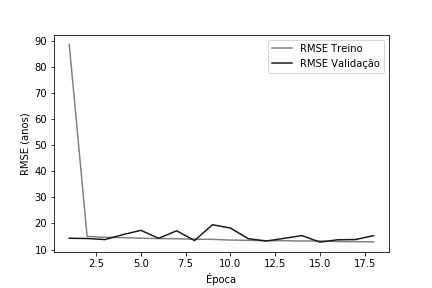
\includegraphics[width=\linewidth]{img/graficos/history/alexnet/fig-history-image-treat-2-alexnet-lrelu-rmse.png}
    \end{subfigure}
    \begin{subfigure}[hb]{0.4\linewidth}
      \caption{Reta-0.}

      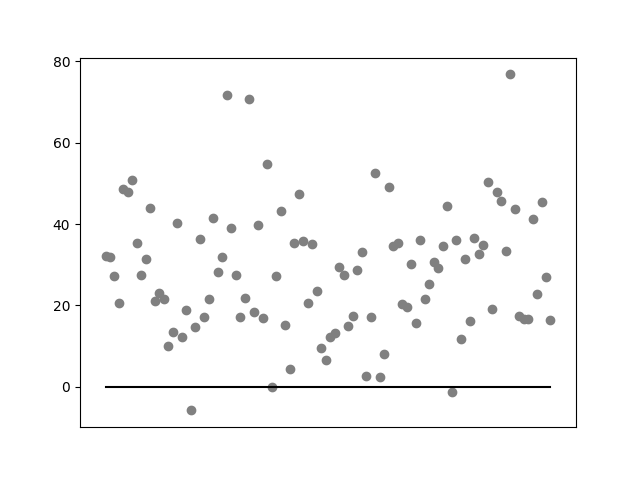
\includegraphics[width=\linewidth]{img/graficos/reta0/alexnet/fig-reta-0-image-treat-2-alexnet-lrelu.png}
    \end{subfigure}%
\end{figure}
\end{frame}

\begin{frame}{Abordagem 2: Introduzindo \emph{Data Augmentation}}
  \begin{table}[!ht]
		\caption{Resultados do treino e teste dos modelos propostos na Abordagem 1.}
		\label{tab:results-1}
		\begin{center}
			\begin{tabular}{l l l l l}
				\toprule
				Rede & Função de ativação & Épocas & MAE Teste & RMSE Teste \\
				\midrule
        LeNet & \emph{ReLU}  & 39 & 37.85 & 40.27 \\
				LeNet & \emph{Leaky ReLU} & 21 & 38.50 & 41.06 \\
				AlexNet & \emph{ReLU}  & 16 & 11.59 & 14.59 \\
				AlexNet & \emph{Leaky ReLU} & 16 & 28.06 & 31.81 \\
				\bottomrule
			\end{tabular}
		\end{center}
	\end{table}
\end{frame}



\begin{frame}{Abordagem 3}
 \begin{itemize}
   \item Entradas: Imagens normalizadas, \alert{equalização por histograma}, \emph{data augmentation}
   \begin{itemize}
     \item Rotação, zoom, inversão horizontal e translação
   \end{itemize}
   \item Redes: LeNet e AlexNet
   \item Funções de ativação: \emph{ReLU} e \emph{Leaky ReLU}
   \end{itemize}
\end{frame}

\begin{frame}{Abordagem 3: Introduzindo Equalização de Histograma}
\begin{figure}[h!]
  \caption{Resultados do treinamento e teste da CNN LeNet \emph{ReLU}.}
  \begin{subfigure}[hb]{0.4\textwidth}
    \caption{RMSE de treinamento.}
    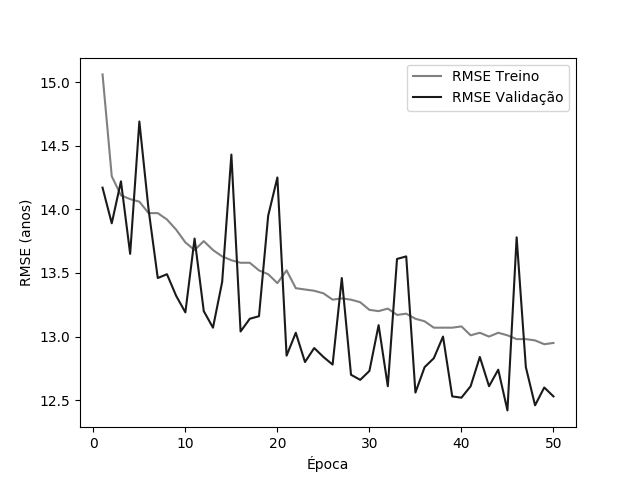
\includegraphics[width=\linewidth]{img/graficos/history/lenet/fig-history-image-treat-3-lenet-relu-rmse.png}%
  \end{subfigure}%
  \begin{subfigure}[hb]{0.4\textwidth}
    \caption{Reta-0 do conjunto de teste.}
    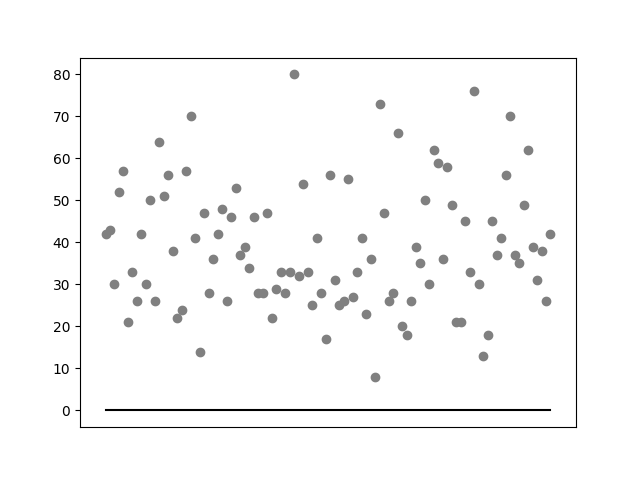
\includegraphics[width=\linewidth]{img/graficos/reta0/lenet/fig-reta-0-image-treat-3-lenet-relu.png}%
  \end{subfigure}
\end{figure}
\end{frame}

\begin{frame}{Abordagem 3: Introduzindo Equalização de Histograma}
  \begin{figure}[h!]
    \caption{Resultados do treinamento e teste da CNN LeNet \emph{Leaky ReLU}.}
  \begin{subfigure}[hb]{0.4\textwidth}
    \caption{RMSE de treinamento.}
    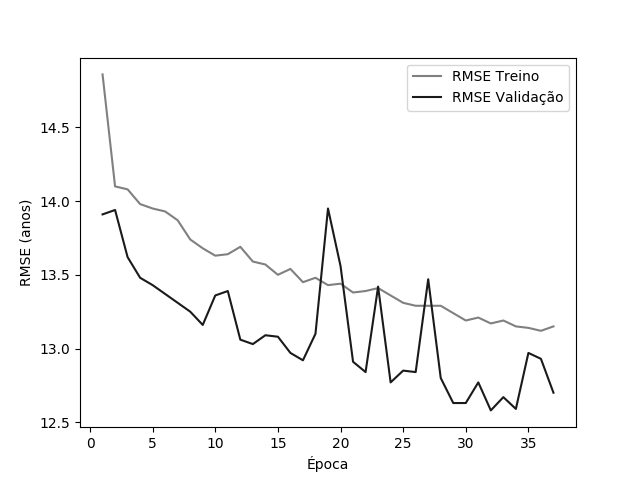
\includegraphics[width=\linewidth]{img/graficos/history/lenet/fig-history-image-treat-3-lenet-lrelu-rmse.png}
  \end{subfigure}
  \begin{subfigure}[hb]{0.4\textwidth}
    \caption{Reta-0 do conjunto de teste.}
   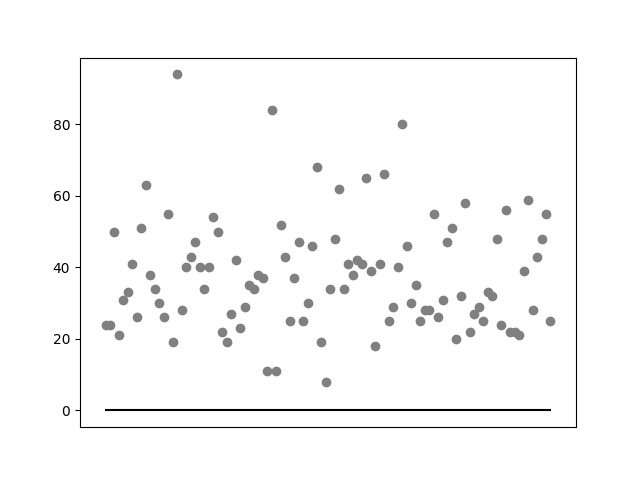
\includegraphics[width=\linewidth]{img/graficos/reta0/lenet/fig-reta-0-image-treat-3-lenet-lrelu.png}
  \end{subfigure}%
\end{figure}
\end{frame}

\begin{frame}{Abordagem 3: Introduzindo Equalização de Histograma}
  \begin{figure}[ht!]
    \caption{Resultados do treinamento e teste da CNN AlexNet \emph{ReLU}.}\label{fig:alexnet-abordagem1}
    \begin{subfigure}[hb]{0.4\linewidth}
      \caption{RMSE Treinamento.}

      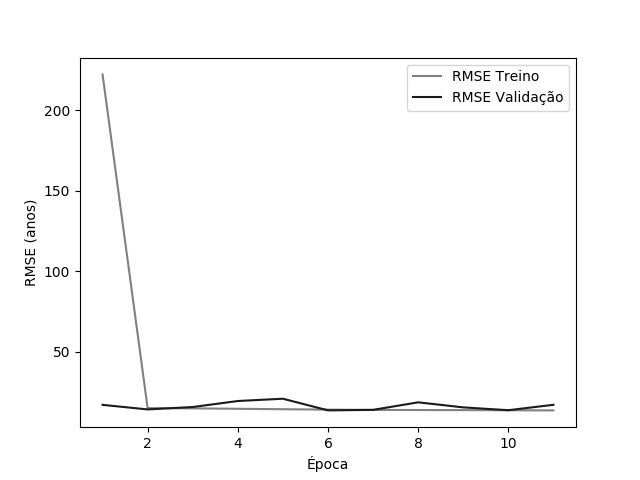
\includegraphics[width=\linewidth]{img/graficos/history/alexnet/fig-history-image-treat-3-alexnet-relu-rmse.png}
    \end{subfigure}
    \begin{subfigure}[hb]{0.4\linewidth}
      \caption{Reta-0.}
      \label{fig:reta0reludying}
      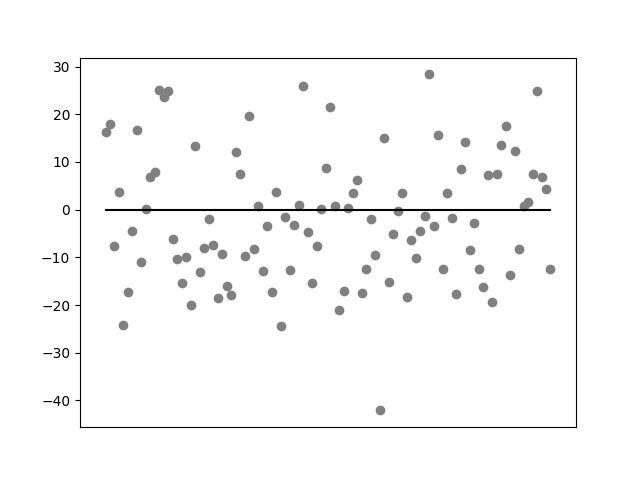
\includegraphics[width=\linewidth]{img/graficos/reta0/alexnet/fig-reta-0-image-treat-3-alexnet-relu.png}%
    \end{subfigure}
\end{figure}
\end{frame}

\begin{frame}{Abordagem 3: Introduzindo Equalização de Histograma}
  \begin{figure}[ht!]
    \caption{Resultados do treinamento e teste da CNN AlexNet \emph{Leaky ReLU}.}\label{fig:alexnet-abordagem1}
    \begin{subfigure}[hb]{0.4\linewidth}
      \caption{RMSE Treinamento.}
      \label{fig:histalexlrelunorm}
      \centering
      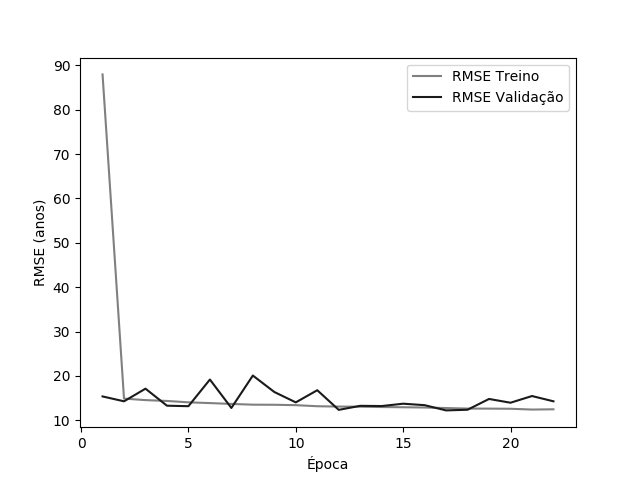
\includegraphics[width=\linewidth]{img/graficos/history/alexnet/fig-history-image-treat-3-alexnet-lrelu-rmse.png}
    \end{subfigure}
    \begin{subfigure}[hb]{0.4\linewidth}
      \caption{Reta-0.}

      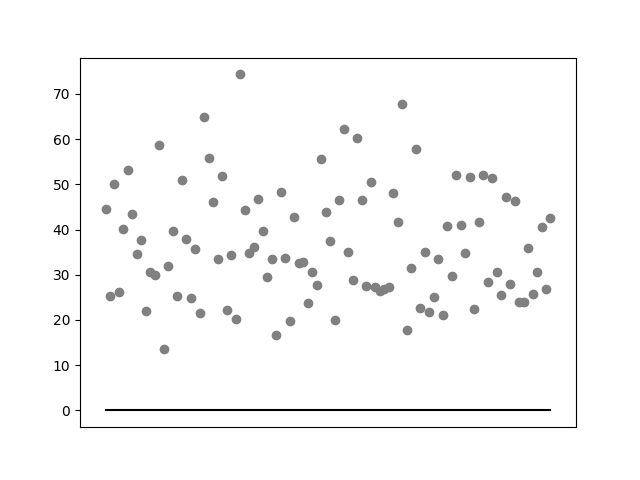
\includegraphics[width=\linewidth]{img/graficos/reta0/alexnet/fig-reta-0-image-treat-3-alexnet-lrelu.png}
    \end{subfigure}%
\end{figure}
\end{frame}

\begin{frame}{Abordagem 3: Introduzindo Equalização de Histograma}
  \begin{table}[!ht]
		\caption{Resultados do treino e teste dos modelos propostos na Abordagem 1.}
		\label{tab:results-1}
		\begin{center}
			\begin{tabular}{l l l l l}
				\toprule
				Rede & Função de ativação & Épocas & MAE Teste & RMSE Teste \\
				\midrule
        LeNet & \emph{ReLU} & 46 &  38.66 & 41.20 \\
				LeNet & \emph{Leaky ReLU} &  38 & 38.26 & 40.85 \\
				AlexNet & \emph{ReLU} & 7 & 13.10 & 15.88 \\
				AlexNet & \emph{Leaky ReLU} & 18 & 35.25 & 38.04 \\
				\bottomrule
			\end{tabular}
		\end{center}
	\end{table}
\end{frame}



\begin{frame}{Abordagem 4}
 \begin{itemize}
   \item Rede com melhor desempenho verificado até então
   \item  \alert{LeNet \emph{ReLU} da Abordagem 1}
   \ \ \newline
   \item Entradas: Imagens normalizadas, equalização por histograma, \emph{data augmentation}
   \item Rede: LeNet
   \item Funções de ativação: \emph{ReLU}
   \ \ \newline
   \item Adoção do MAE para cálculo da perda
   \item Tamanho do batch alterado para 128 imagens
   \end{itemize}
\end{frame}

\begin{frame}{Abordagem 4: Utilizando MAE para o Cálculo da Perda}
  \begin{figure}[hb!]
		\caption{Resultados do treinamento e teste da CNN LeNet de acordo com a Abordagem 4.}\label{fig:lenet-abordagem4}
		\begin{subfigure}[hb]{0.5\linewidth}
			\caption{MAE de treinamento}
			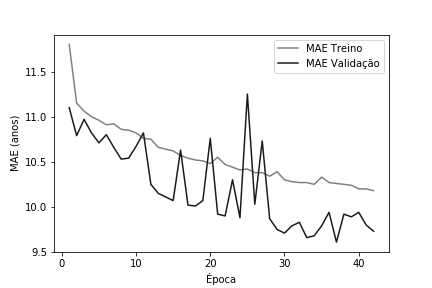
\includegraphics[width=\linewidth]{img/graficos/history/lenet/fig-history-abordagem-4-lenet-relu-mae.png}%
		\end{subfigure}%
		\begin{subfigure}[hb]{0.5\linewidth}
			\caption{Reta-0}
			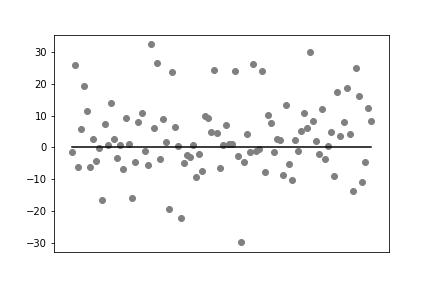
\includegraphics[width=\linewidth]{img/graficos/reta0/lenet/fig-reta-0-abordagem-4-lenet-relu.png}%
		\end{subfigure}
	\end{figure}
\end{frame}

\begin{frame}{Abordagem 4: Utilizando MAE para o Cálculo da Perda}
  \begin{table}[!ht]
		\caption{Resultados do treino e teste do modelo proposto na Abordagem 4.}
		\label{tab:results-1}
		\begin{center}
			\begin{tabular}{l l l l l}
				\toprule
				Rede & Função de ativação & Épocas & MAE Teste & RMSE Teste \\
				\midrule
        LeNet & \emph{Leaky ReLU} & 38 & 9.98 & 12.91 \\
				\bottomrule
			\end{tabular}
		\end{center}
	\end{table}
\end{frame}



\begin{frame}{Abordagem 5}
 \begin{itemize}
   \item Rede com melhor desempenho verificado até então
   \item  \alert{LeNet \emph{ReLU} da Abordagem 1}
   \ \ \newline
   \item Entradas: \alert{Imagens normalizadas}
   \item Rede: LeNet
   \item Funções de ativação: \emph{ReLU}
   \ \ \newline
   \item Cálculo da perda considerando o MAE
   \item Tamanho do batch: 128 imagens
   \end{itemize}
\end{frame}

\begin{frame}{Abordagem 5: LeNet Apenas com Normalização da Entrada}
  \begin{figure}[hb!]
		\caption{Resultados do treinamento e teste da CNN LeNet de acordo com a Abordagem 5.}\label{fig:lenet-abordagem4}
		\begin{subfigure}[hb]{0.5\linewidth}
			\caption{MAE de treinamento}
			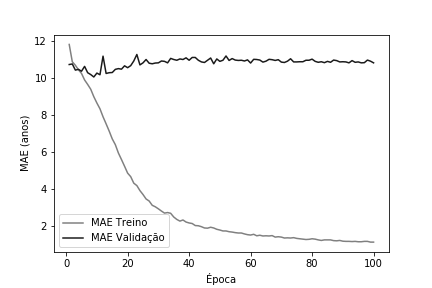
\includegraphics[width=\linewidth]{img/graficos/history/lenet/fig-history-abordagem-5-lenet-relu-mae.png}%
		\end{subfigure}%
		\begin{subfigure}[hb]{0.5\linewidth}
			\caption{Reta-0}
			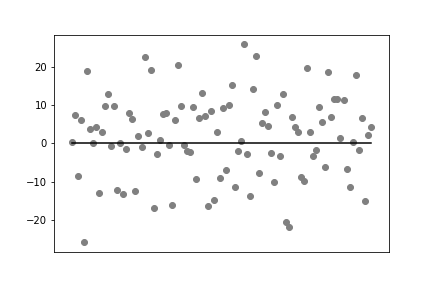
\includegraphics[width=\linewidth]{img/graficos/reta0/lenet/fig-reta-0-abordagem-5-lenet-relu.png}%
		\end{subfigure}
	\end{figure}
\end{frame}

\begin{frame}{Abordagem 5: LeNet Apenas com Normalização da Entrada}
  \begin{table}[!ht]
		\caption{Resultados do treino e teste do modelo proposto na Abordagem 5.}
		\label{tab:results-1}
		\begin{center}
			\begin{tabular}{l l l l l}
				\toprule
				Rede & Função de ativação & Épocas & MAE Teste & RMSE Teste \\
				\midrule
        LeNet & \emph{ReLU} & 9 &  10.09 & 13.04 \\
				\bottomrule
			\end{tabular}
		\end{center}
	\end{table}
\end{frame}



\begin{frame}{Abordagem 6}
 \begin{itemize}
   \item Entradas: Imagens normalizadas
   \item Rede: \alert{VGG-16}
   \item Funções de ativação: \emph{ReLU}
   \ \ \newline
   \item Cálculo da perda considerando o MAE
   \item \alert{Tamanho do batch: 64 imagens}
   \end{itemize}
\end{frame}

\begin{frame}{Abordagem 6: VGG-16 e Dados Normalizados}
  \begin{figure}[hb!]
    \caption{Resultados do treinamento e teste da CNN VGG-16 de acordo com a Abordagem 6.}\label{fig:vgg-abordagem6}
    \begin{subfigure}[hb]{0.5\linewidth}
      \caption{MAE de treinamento da arquitetura VGG-16 utilizando funções de ativação \emph{ReLU}.}
      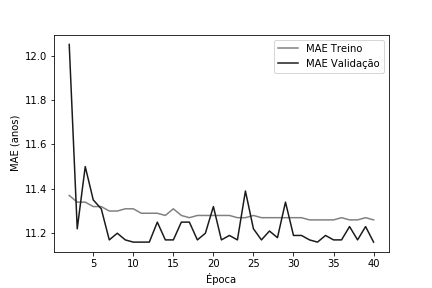
\includegraphics[width=\linewidth]{img/graficos/history/vgg16/fig-history-abordagem6-vgg16-relu-mae.png}%
    \end{subfigure}%
    \begin{subfigure}[hb]{0.5\linewidth}
      \caption{Reta-0 VGG-16 \emph{ReLU}.}
      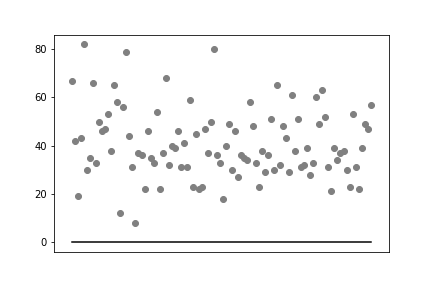
\includegraphics[width=\linewidth]{img/graficos/reta0/vgg16/fig-reta-0-abordagem6-vgg16-relu.png}%
    \end{subfigure}\\
  \end{figure}
\end{frame}

\begin{frame}{Abordagem 6: VGG-16 e Dados Normalizados}
  \begin{table}[!ht]
    \centering
    \caption{Resultados do treino e teste dos modelos propostos na Abordagem 6.}
    \label{tab:results-6}
    \begin{tabular}{l l l l l l l}
      \toprule
      Rede & Função de ativação & Épocas & MAE Teste & RMSE Teste \\
      \midrule
      VGG-16 & \emph{ReLU} & 11 & 40.90 & 38.35 \\
      \bottomrule
    \end{tabular}
  \end{table}
\end{frame}

\begin{frame}{Abordagem 6: VGG-16 e Dados Normalizados}
  \begin{itemize}
    \item \emph{Dying ReLU problem}
    \item Saídas iguais a $37.05$ para todas as imagens dadas como entrada
  \end{itemize}
\end{frame}




\begin{frame}{Abordagem 7}
 \begin{itemize}
   \item Entradas: Imagens normalizadas, \alert{equalização por histograma, \emph{data augmentation}}
   \item Rede: VGG-16
   \item Funções de ativação: \emph{ReLU}
   \ \ \newline
   \item Cálculo da perda considerando o MAE
   \item Tamanho do batch: 64 imagens
   \end{itemize}
\end{frame}

\begin{frame}{Abordagem 7: VGG-16 com \emph{Data Augmentation} e Equalização de Histograma}
  \begin{figure}[h!]
    \caption{Resultados do treinamento e teste da CNN VGG-16 de acordo com a Abordagem 7.}\label{fig:vgg-abordagem7}
    \begin{subfigure}[hb]{0.5\linewidth}
      \caption{MAE de treinamento da arquitetura VGG-16 utilizando funções de ativação \emph{ReLU}.}
      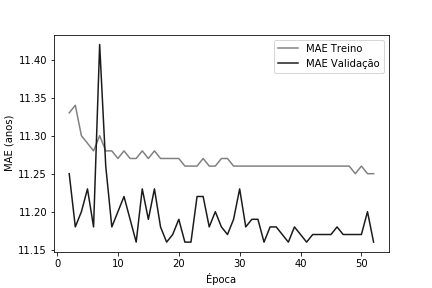
\includegraphics[width=\linewidth]{img/graficos/history/vgg16/fig-history-abordagem7-vgg16-relu-mae.png}%
    \end{subfigure}%
    \begin{subfigure}[hb]{0.5\linewidth}
      \caption{Reta-0 VGG-16 \emph{ReLU}.}
      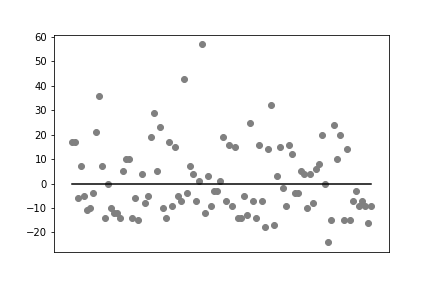
\includegraphics[width=\linewidth]{img/graficos/reta0/vgg16/fig-reta-0-abordagem7-vgg16-relu.png}%
    \end{subfigure}\\
  \end{figure}
\end{frame}

\begin{frame}{Abordagem 7: VGG-16 com \emph{Data Augmentation} e Equalização de Histograma}
  \begin{table}[!ht]
  	\centering
  	\caption{Resultados do treino e teste dos modelos propostos na Abordagem 7.}
  	\label{tab:results-7}
  		\begin{tabular}{l l l l l }
  			\toprule
  			Rede & Função de ativação & Épocas & MAE Teste & RMSE Teste \\
  			\midrule
  			VGG-16 & \emph{ReLU} & 23 & 40.99 & 38.39 \\
  			\bottomrule
  		\end{tabular}
  	\end{table}
\end{frame}

\begin{frame}{Abordagem 7: VGG-16 com \emph{Data Augmentation} e Equalização de Histograma}
  \begin{itemize}
    \item \emph{Dying ReLU problem}
    \item Saídas iguais a $37.02$ para todas as imagens dadas como entrada
  \end{itemize}
\end{frame}



\begin{frame}{Abordagem 8}
 \begin{itemize}
   \item Entradas: Imagens normalizadas, equalização por histograma, \emph{data augmentation}
   \item Rede: VGG-16
   \item Função de ativação na camada de saída: \alert{\emph{Leaky ReLU}}
   \item \alert{\emph{Transfer Learning}: ImageNet}
   \ \ \newline
   \item Cálculo da perda considerando o MAE
   \item Tamanho do batch: 64 imagens
   \end{itemize}
\end{frame}

\begin{frame}{Abordagem 8: VGG-16 com \emph{data augmentation}, \emph{Transfer Learning} e \emph{Leaky ReLU}}
  \begin{figure}[h!]
    \caption{Resultados do treinamento e teste da CNN VGG-16 de acordo com a Abordagem 8.}\label{fig:vgg-abordagem8}
    \begin{subfigure}[hb]{0.5\linewidth}
      \caption{MAE de treinamento da arquitetura VGG-16 utilizando funções de ativação \emph{Leaky ReLU}.}
      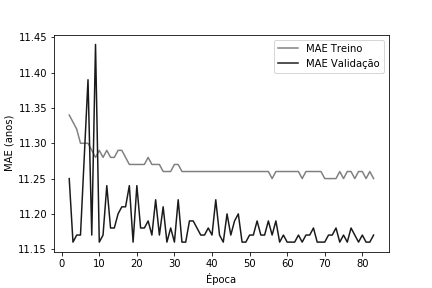
\includegraphics[width=\linewidth]{img/graficos/history/vgg16/fig-history-abordagem9-vgg16-lrelu-mae.png}%
    \end{subfigure}%
    \begin{subfigure}[hb]{0.5\linewidth}
      \caption{Reta-0 VGG-16 \emph{Leaky ReLU}.}
      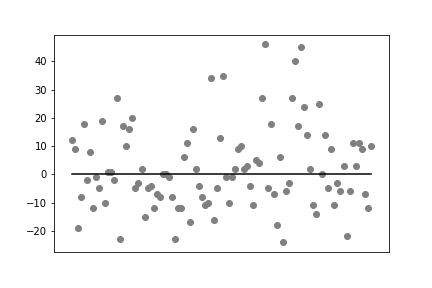
\includegraphics[width=\linewidth]{img/graficos/reta0/vgg16/fig-reta-0-abordagem9-vgg16-lrelu.png}%
    \end{subfigure}\\
  \end{figure}
\end{frame}

\begin{frame}{Abordagem 8: VGG-16 com \emph{data augmentation}, \emph{Transfer Learning} e \emph{Leaky ReLU}}
  \begin{table}[!ht]
  \centering
  \caption{Resultados do treino e teste dos modelos propostos na Abordagem 8.}
  \label{tab:results-8}
   \begin{tabular}{l l l l l }
  	 \toprule
  	 Rede & Função de ativação & Épocas & MAE Teste & RMSE Teste \\
  	 \midrule
  	 VGG-16 & \emph{Leaky ReLU} & 83 & 11.02 & 14.24 \\
  	 \bottomrule
   \end{tabular}
 \end{table}
\end{frame}

\begin{frame}{Abordagem 8: VGG-16 com \emph{data augmentation}, \emph{Transfer Learning} e \emph{Leaky ReLU}}
  \begin{itemize}
    \item \emph{Dying ReLU problem}
    \item Saídas iguais a $36.99$ para todas as imagens dadas como entrada
  \end{itemize}
\end{frame}




\begin{frame}{Abordagem 9}
 \begin{itemize}
   \item Entradas: Imagens normalizadas, equalização por histograma, \emph{data augmentation}
   \item Rede: \alert{SqueezeNet}
   \item Função de ativação na camada de saída: \emph{ReLU}
   \ \ \newline
   \item Cálculo da perda considerando o MAE
   \item Tamanho do batch: 64 imagens
   \end{itemize}
\end{frame}
%
\begin{frame}{Abordagem 9: SqueezeNet}
  \begin{figure}[h!]
		\caption{Resultados do treinamento e teste da CNN SqueezeNet de acordo com a Abordagem 9.}\label{fig:squeeze-abordagem9}
		\begin{subfigure}[hb]{0.5\linewidth}
			\caption{MAE de treinamento da arquitetura SqueezeNet utilizando função de ativação \emph{ReLU} e \emph{data augmentation}.}
			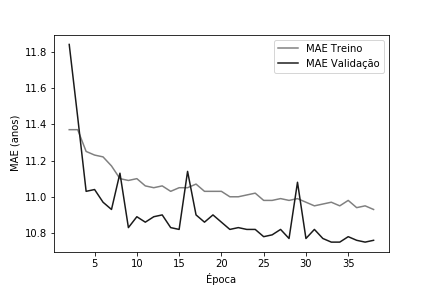
\includegraphics[width=\linewidth]{img/graficos/history/squeeze/fig-history-abordagem-squeeze1-squeeze-relu-mae.png}%
		\end{subfigure}%
		\begin{subfigure}[hb]{0.5\linewidth}
			\caption{Reta-0 SqueezeNet.}
			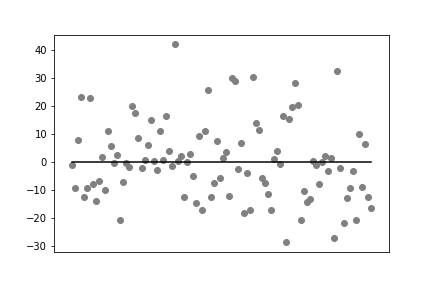
\includegraphics[width=\linewidth]{img/graficos/reta0/squeeze/fig-reta-0-abordagem-squeeze1-squeeze-relu.png}%
		\end{subfigure}\\
	\end{figure}
\end{frame}

\begin{frame}{Abordagem 9: SqueezeNet}
  \begin{table}[!ht]
	\centering
	\caption{Resultado do teste da SqueezeNet proposta na Abordagem 9.}
	\label{tab:results-9}
		\begin{tabular}{l l l l l }
			\toprule
			Rede & Função de ativação & Épocas & MAE Teste & RMSE Teste \\
			\midrule
			SqueezeNet & \emph{ReLU} & 38 & 10.72 & 13.84 \\
			\bottomrule
		\end{tabular}
	\end{table}
\end{frame}



\begin{frame}{Sumarizando os Resultados}
  \begin{table}[b]
	\caption{Sumário dos resultados obtidos de todas as abordagens conduzidas.}
	\label{tab:resultsAll}
  \begin{center}
	\resizebox{0.68\linewidth}{!} {
		\begin{tabular}{cccccc}
			\toprule
			Abordagem & Rede & Função de ativação & Épocas & MAE Teste & RMSE Teste \\
			\midrule
			1 & LeNet & \emph{ReLU}  & 4 & 10.53 & 13.55 \\
			1 & LeNet & \emph{Leaky ReLU} & 8 & 38.33 & 40.82 \\
			1 & AlexNet & \emph{ReLU}  & 5 & 11.03 & 13.76 \\
			1 & AlexNet & \emph{Leaky ReLU} & 5 & 39.27 & 41.97 \\
			2 & LeNet & \emph{ReLU}  & 39 & 37.85 & 40.27 \\
			2 & LeNet & \emph{Leaky ReLU} & 21 & 38.50 & 41.06 \\
			2 & AlexNet & \emph{ReLU}  & 16 & 11.59 & 14.59 \\
			2 & AlexNet & \emph{Leaky ReLU} & 16 & 28.06 & 31.81 \\
			3 & LeNet & \emph{ReLU} & 46 &  38.66 & 41.20 \\
			3 & LeNet & \emph{Leaky ReLU} &  38 & 38.26 & 40.85 \\
			3 & AlexNet & \emph{ReLU} & 7 & 13.10 & 15.88 \\
			3 & AlexNet & \emph{Leaky ReLU} & 18 & 35.25 & 38.04 \\
			4 &	LeNet & \emph{Leaky ReLU} & 38 & 9.98 & 12.91 \\
			5 & LeNet & \emph{ReLU} & 9 &  10.09 & 13.04 \\
			6 & VGG-16 & \emph{ReLU} & 11 & 40.90 & 38.35 \\
			7 & VGG-16 & \emph{ReLU} & 23 & 40.99 & 38.39 \\
			8 & VGG-16 & \emph{Leaky ReLU} & 83 & 11.02 & 14.24 \\
			9 & SqueezeNet & \emph{ReLU} & 38 & 10.72 & 13.84 \\
			\bottomrule
		\end{tabular}
		}
  \end{center}
\end{table}

\end{frame}
